\section{Projektsamarbejde}
\label{ProjektSamarbejde}
%
Projektet dækker over et samarbejde mellem projektgruppen, inklusiv vejleder, og Karl Damkjær Hansens, som er ansat ved Aalborg Universitet. Karls arbejde involverer udviklingen af sociale robotter, som skal indgå i en menneske-robot interaktion, \textit{Human-Robot Interaction}, HRI. Dertil fokuseres der på, hvordan den sociale robot skal henvende sig til interaktionspartneren(e), hvor Karl's primære arbejdsområde dækker det tekniske aspekt. Da sociale robotter skal kunne indgå i HRI er det en fordel at robotten afspejler menneskelig adfærd, eksempelvis i forhold til bevægelsesmønstre, hvor målet dels er at få robotten til at udføre dynamiske bevægelser og dels tillade robotten friheden til at bevæge sig 360$^{\circ}$. Ved at opfylde de to mål bør det være muligt at få robotten til at gengive menneskelige bevægelser såsom vægtfordeling under en stående samtale samt øge samtalekredsen for at inkludere én eller flere samtalepartnere.

For at muliggøre dette arbejder Karl med at udvikle en robot, som balancerer på en kugle (FIND UD AF HVOR STOR KUGLEN ER!), hvilket tillader 360$^{\circ}$ bevægelse, og i tillæg benyttes inerti til at gengive menneskelige bevægelser. Robotten illustreres på \autoref{fig:VoresRobot}. Ved at balancere robotten på en kugle gør det, det muligt ikke blot at bevæge sig frem og tilbage men også sidelæns, hvilket eksempelvis ikke er tilfældet ved \textit{Double}, \parencite{WEB:Double}, som balancerer på en cylinder, hvilket er illustreret på \autoref{fig:Double}. Fælles for Karl's robot og \textit{Double} er, at de begge benytter sig inerti, for at gengive menneskelige bevægelser, såsom vægtfordeling. Kuglens store diameter tillader robotten at køre ubesværet og naturligt på de fleste overflader og i tilfæde hvor robotten skal køre over et dørtrin, så vil det fremstå flydende og ikke skramlende, som er tilfældet ved en mindre kugle diameter. 
%
\begin{figure}[H]
\centering
\begin{minipage}{.5\textwidth}
  \centering
  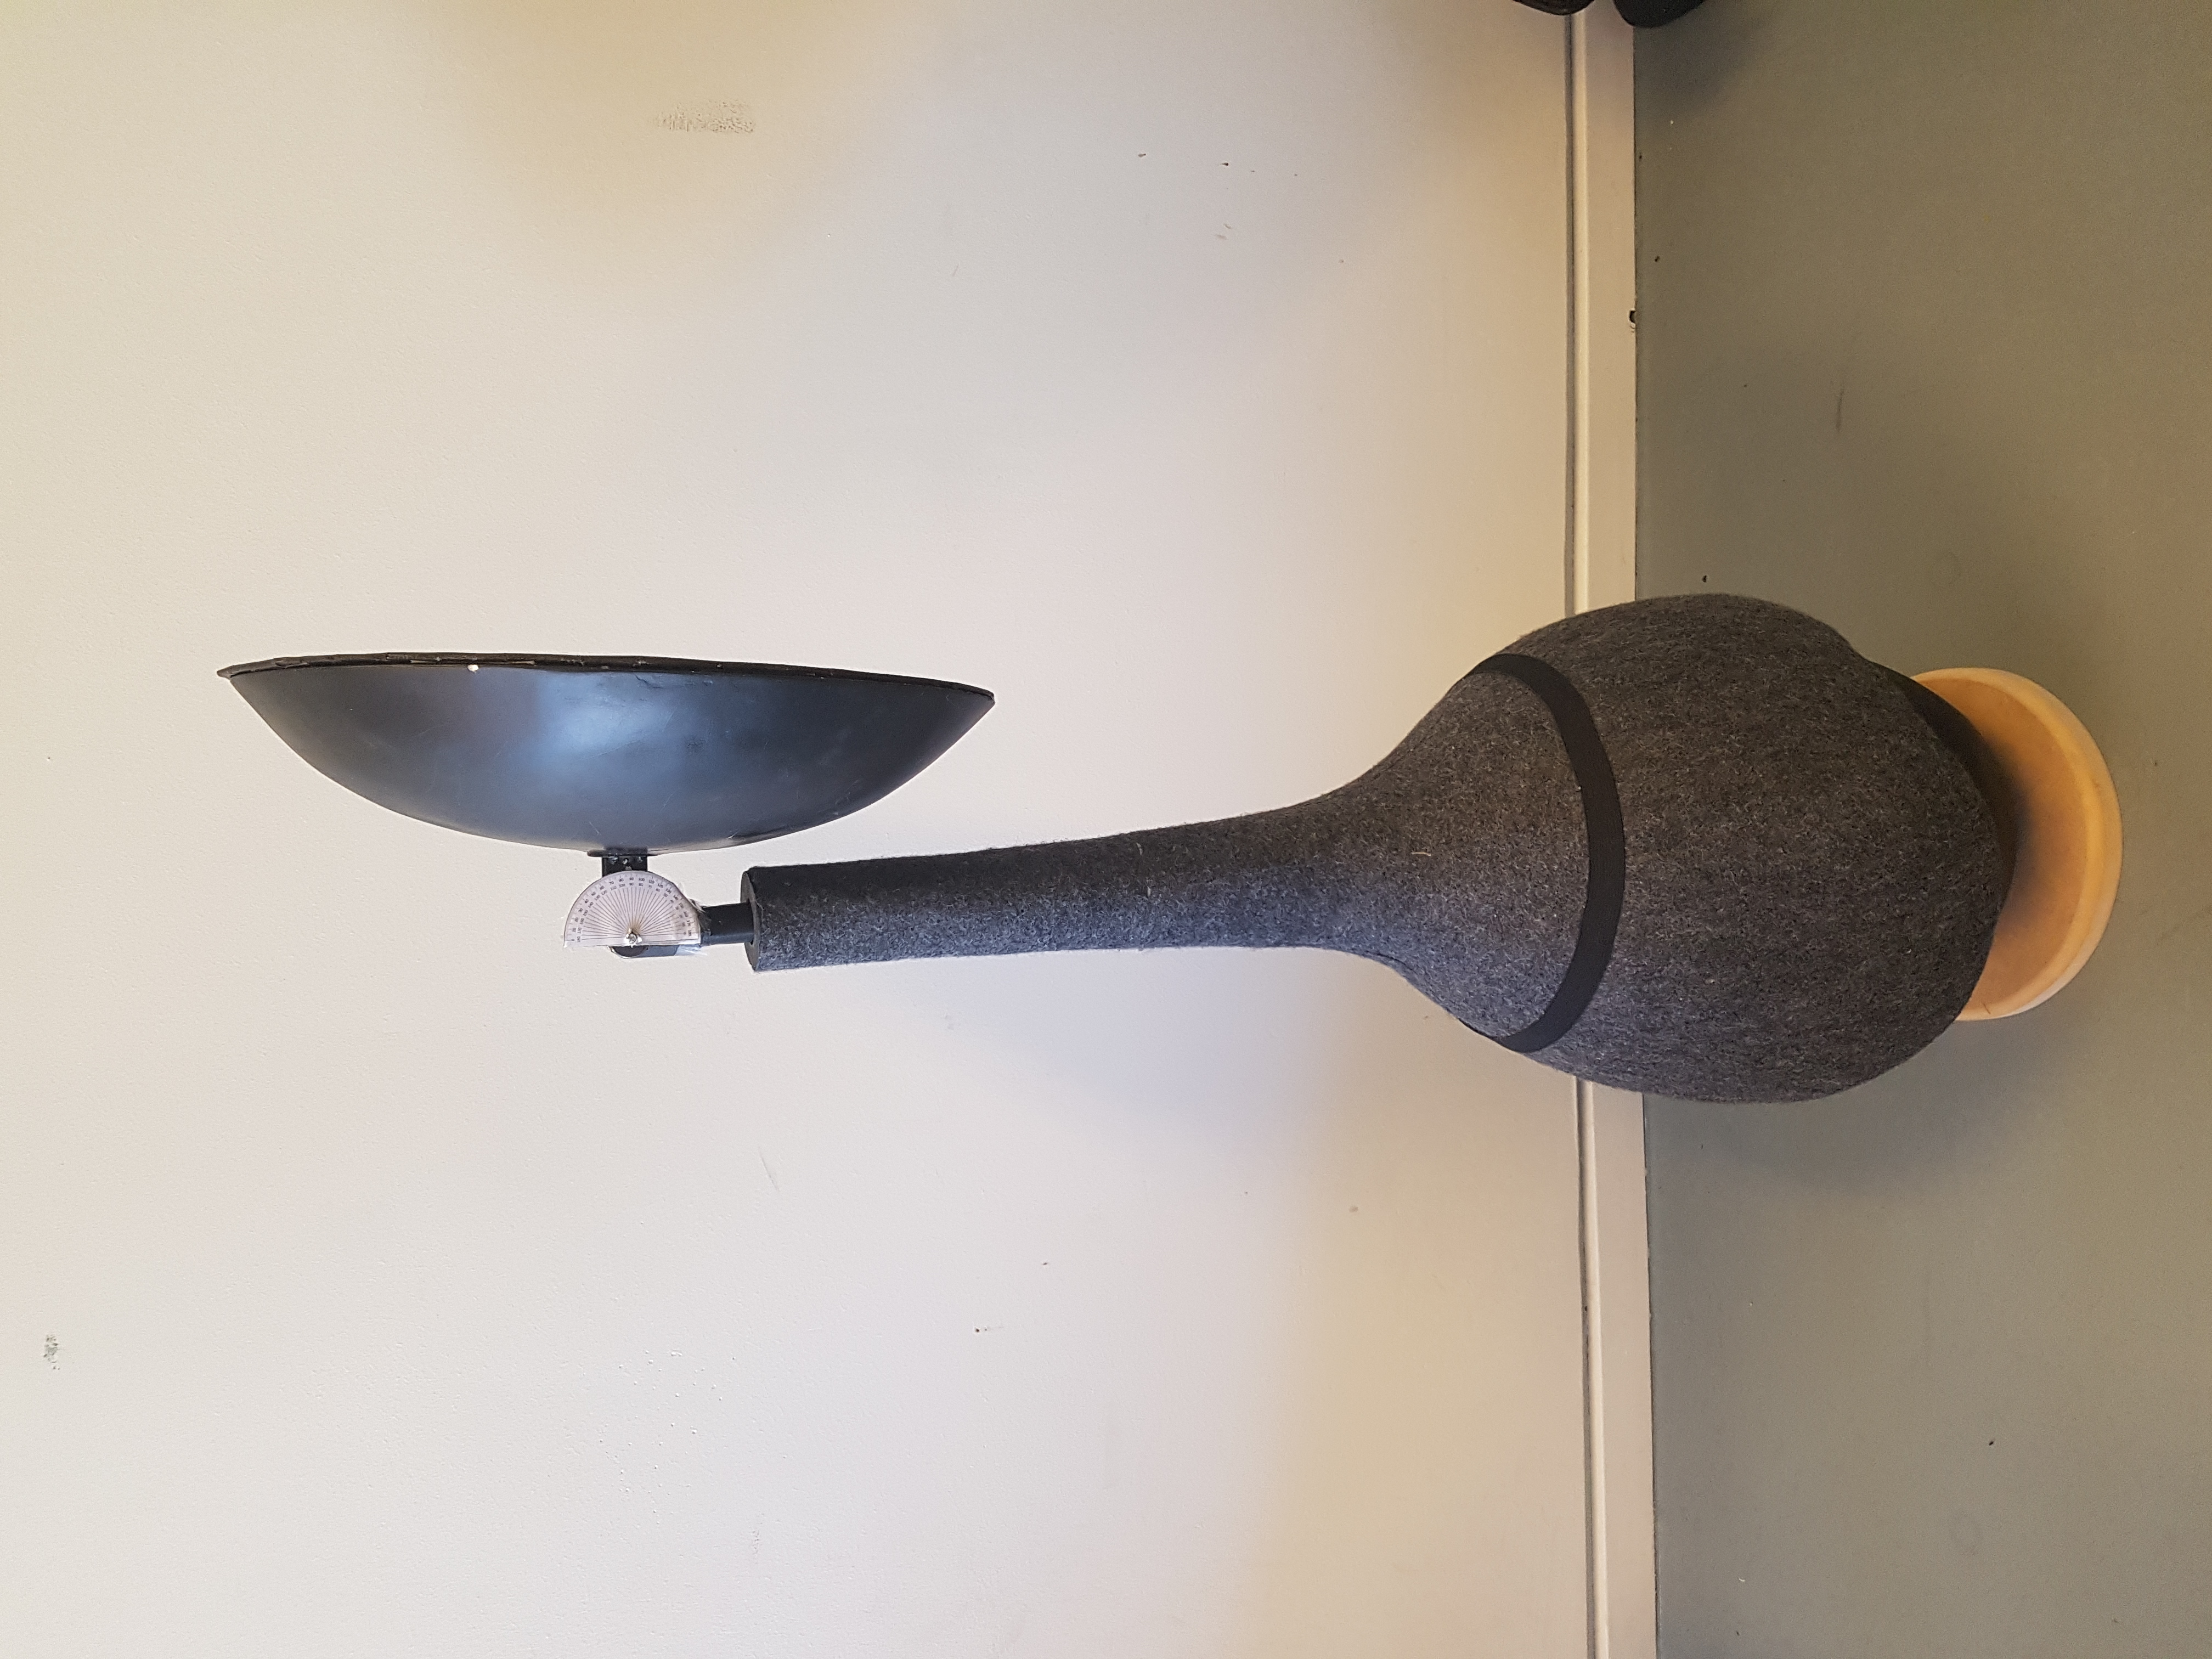
\includegraphics[width=.8\linewidth, angle =-90]{Figure/TEST.jpg}
  \caption{FIND ET ANDET BILLEDE}
  \label{fig:VoresRobot}
\end{minipage}%
\begin{minipage}{.5\textwidth}
  \centering
  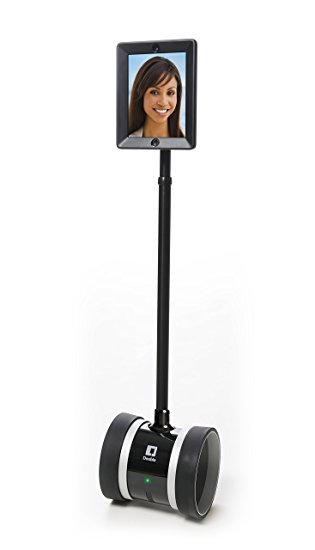
\includegraphics[width=.48\linewidth]{Figure/Double}
  \caption{Illustration af \textit{Double}, \parencite{WEB:Double}.}
  \label{fig:Double}
\end{minipage}
\end{figure}
\noindent
%
Formålet med robotten er, at den skal indgå i Københavns Lufthavn, hvor den eksempelvis skal hjælpe de rejsende med at finde frem til deres gate i tide. At robotten skal indgå i Københavns Lufthavn udspringer fra samarbejdet mellem Karl, Combine og Københavns Lufthavn. De udviklere og designere, som Karl har været i kontakt med, giver udtryk for ikke at være interesserede i, hvordan robotten bevæger sig. De foretrækker at robotten har nogle foruddefinerede indstillinger for den grundlæggende måde hvorpå robotten bevæger sig, hvilket skal stemme overens med, hvad der forventes af en social robot. Derfor handler projektet for Karl om, at få robotten til at bevæge sig på en hensigtmæssig måde, så det er muligt for den at indgå i HRI. Det er med udgangpunkt i dette, projektsamarbejdet med Karl udspringer. 

Det overordnede formål med dette projekt er derfor, at undersøge dels hvordan robotten skal bevæge sig for at indgå i den sociale kontekst; Københavns Lufthavn, og dels hvordan den rejsendes subjektive oplevelse af interaktion er.\blankline
%  
For at udvikle den sociale intelligens i robotten; hvordan robotten skal agere og reagere blandt mennesker, er det nødvendigt at undersøge hvilke parametre, der har indflydelse på den subjektive oplevelse af HRI. I følgende afsnit undersøges eksisterende sociale robotter, der allerede er på markedet, interaktion med sociale robotter, herunder hvilke parametre der har indflydelse på denne og efterfølgende undersøges udfordringer ved sociale robotter. SKRIV IND NÅR DET ER BESLUTTET HVOR DET OM LUFTHAVNEN SKAL VÆRE HENNE.   

